\documentclass[10pt,twocolumn,letterpaper]{article}

\usepackage{cvpr}
\usepackage{times}
\usepackage{epsfig}
\usepackage{graphicx}
\usepackage{amsmath}
\usepackage{amssymb}
\usepackage{booktabs}

\usepackage[breaklinks=true,bookmarks=false]{hyperref}

% Float placement: let LaTeX fill more of each page with figures so
% they land near their in-text reference rather than piling up at the
% end. Defaults (0.7/0.2) are too conservative for figure-heavy
% short papers.
\renewcommand{\topfraction}{0.9}
\renewcommand{\bottomfraction}{0.9}
\renewcommand{\textfraction}{0.07}
\renewcommand{\floatpagefraction}{0.75}
\setcounter{topnumber}{3}
\setcounter{bottomnumber}{2}
\setcounter{totalnumber}{5}

\cvprfinalcopy
\def\cvprPaperID{****}
\def\httilde{\mbox{\tt\raisebox{-.5ex}{\symbol{126}}}}

\setcounter{page}{1}
\begin{document}

%%%%%%%%% TITLE
\title{PhantomMap: A First-Party Atlas of Where Vision--Language Models Place Objects That Don't Exist}

\author{%
  Shouyu Wang \\
  Rice University\\
  {\tt\small sw188@rice.edu}
  \and
  Limeng Wang \\
  Rice University\\
  {\tt\small lw158@rice.edu}
}

\maketitle

%%%%%%%%% ABSTRACT
\begin{abstract}
   Vision--language models such as Qwen2.5-VL-7B-Instruct
   \cite{qwen25vl} and LLaVA-NeXT-Mistral-7B \cite{llavanext}
   hallucinate objects absent from the input. Prior work diagnoses
   this either by probing internal attention \cite{eazy,opera,halloc}
   or by querying an external detector \cite{woodpecker}. We take a
   complementary angle: the \emph{first-party readout}. When a VLM
   hallucinates, we simply ask it -- through its public prompt
   interface -- to draw a bounding box around the phantom, and analyse
   the resulting boxes at scale. Across $18{,}000$ (image, object)
   probes on three POPE \cite{pope} splits for two models, we collect
   $2{,}806$ phantom bounding boxes and show that they lie
   $20\%$--$32\%$ further from the image centre and cover
   $21\%$--$37\%$ less area than boxes drawn for real objects.
   A logistic regression over eight shape and logit features of the
   phantom box -- trainable in seconds on a CPU -- reaches
   $\mathrm{AUROC}=0.916$ on Qwen2.5-VL and $0.873$ on LLaVA-NeXT,
   both exceeding the internal-feature HALP baseline of $0.787$
   \cite{halp} despite requiring nothing beyond the VLM's API. Where a
   hallucination is drawn turns out to be at least as informative as
   what it names.
\end{abstract}

%%%%%%%%% INTRO
\section{Introduction}

Object hallucination is the most-cited failure mode of modern
multimodal systems \cite{hallsurvey,pope}. Two research traditions
have emerged. \emph{Internal probes} (EAZY \cite{eazy}, OPERA
\cite{opera}, HalLoc \cite{halloc}) open the model to analyse
image-token attention or output-token confidence. \emph{External
verifiers} (Woodpecker \cite{woodpecker}) forward the VLM's caption to
an object detector and flag unconfirmable entities. Both views are
powerful, but neither matches what an end user actually sees.

An end user only sees the VLM's public output. When the output asserts
an object is in the image, a natural follow-up is \emph{``where,
specifically, is it?''} Modern grounded VLMs \cite{qwen25vl} answer
with a bounding box. When the object is absent, the bounding box is a
\emph{phantom}.

This paper contributes: \textbf{(i)} a first-party \emph{spatial
atlas} of $2{,}806$ phantom and $4{,}971$ honest boxes collected from
Qwen2.5-VL-7B-Instruct and LLaVA-NeXT-Mistral-7B on the three POPE
splits -- phantom boxes consistently lie further from the image centre
and are smaller than honest boxes, across both models; and
\textbf{(ii)} a training-free logistic-regression detector over eight
shape/location/logit features of the phantom box, reaching
$\mathrm{AUROC}=0.916$ on Qwen2.5-VL and $0.873$ on LLaVA-NeXT, both
above the internal-feature HALP baseline of $0.787$ \cite{halp}.
Fig.~\ref{fig:teaser} gives the flavour at a glance.

\begin{figure}[!htbp]
\centering
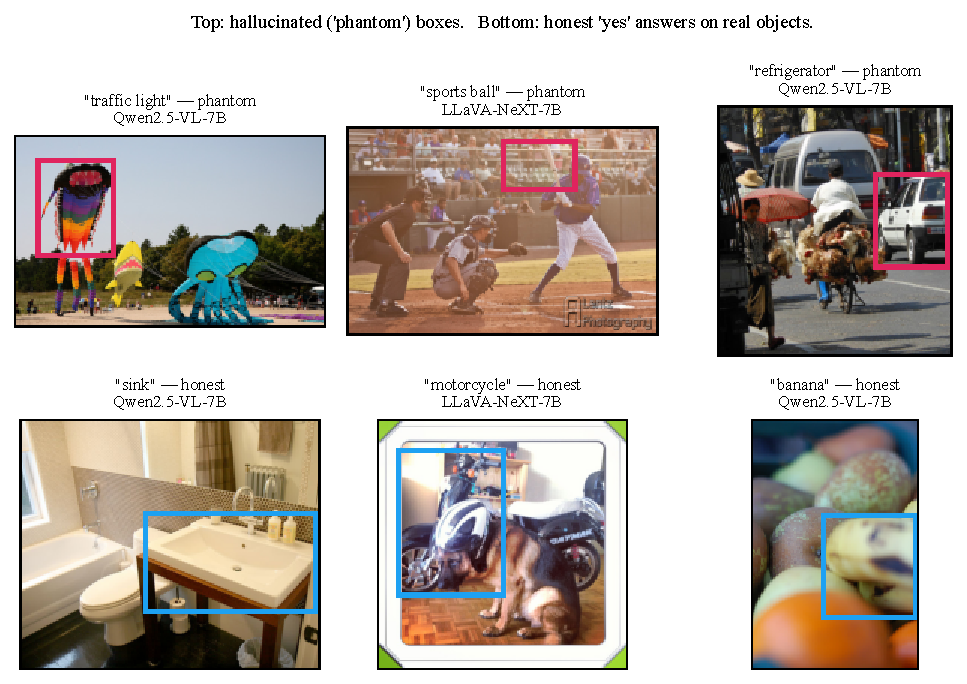
\includegraphics[width=\columnwidth]{figures/fig1_teaser.pdf}
\caption{Phantom boxes (top, objects absent) vs.\ honest boxes
(bottom, objects present) from Qwen2.5-VL and LLaVA-NeXT on POPE.}
\label{fig:teaser}
\end{figure}

\begin{figure*}[!tb]
\centering
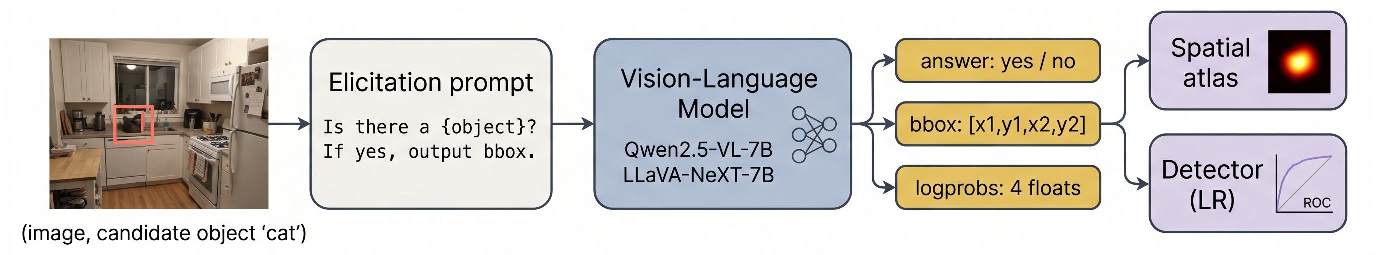
\includegraphics[width=0.95\textwidth]{figures/fig2_method.pdf}
\caption{PhantomMap pipeline. Each $(I, o)$ probe produces a yes/no
answer plus -- on ``yes'' -- a bbox. When POPE labels $o$ absent,
every ``yes'' is a phantom event whose bbox feeds the atlas and the
detector.}
\label{fig:method}
\end{figure*}

%%%%%%%%% RELATED WORK
\section{Related Work}

\paragraph{Benchmarks.} POPE \cite{pope} formalised object
hallucination as a yes/no existence probe on COCO \cite{mscoco}, with
three negative-mining splits (random, popular, adversarial). AMBER
\cite{amber} extends the task to multi-dimensional attribute queries.
Neither asks a VLM \emph{where} a hallucinated object is.

\paragraph{Internals and external verifiers.} EAZY \cite{eazy} traces
hallucinated tokens back to $\sim 3$ high-attention image patches and
zeroes them out. OPERA \cite{opera} penalises an ``over-trust''
attention sink at decode time. HalLoc \cite{halloc} localises
hallucinations at the output text-token level. All three require
model internals. Woodpecker \cite{woodpecker} chains the VLM with
Grounding DINO and flags unverifiable mentions -- trading one oracle
for another.

\paragraph{Feature-based detection.} HALP \cite{halp} trains a
classifier on the VLM's internal visual features and reaches
$\mathrm{AUROC}=0.787$ on Qwen2.5-VL, the strongest published Qwen
baseline we are aware of. DASH \cite{dash} clusters \emph{images}
that systematically trigger hallucinations, complementing our
token-level view with an image-level one. Visual CounterFact
\cite{pixelsvspriors} studies the pixel-vs-prior conflict when the
image contradicts world knowledge.

\paragraph{Grounded VLMs and localisation.} The emergence of
grounded VLMs such as Qwen2.5-VL~\cite{qwen25vl} has elevated object
localisation from an auxiliary capability to a first-class skill,
exposed through a public JSON-bbox interface that any downstream
application can read. Evaluation has largely focused on whether the
model points to the \emph{right} thing (RefCOCO-style benchmarks),
leaving the question of where a grounded VLM points to the
\emph{wrong} thing -- i.e.\ its phantoms -- essentially unstudied.
PhantomMap fills that gap.

Unlike all of the above, PhantomMap operates on the VLM's
\emph{prompted bbox output} -- the channel actually exposed to a
user via the public API -- and is the first to profile the
\emph{spatial distribution} of hallucinated objects in pixel space.
This makes the approach cheap (no model internals, no external
detectors) and portable (any grounded VLM with an API supports it
out of the box).

%%%%%%%%% METHOD
\section{Method}

\paragraph{Elicitation prompt.} For every (image $I$, query object
$o$) we issue one fixed prompt (Fig.~\ref{fig:method}):
``Look at the image. Is there a $\{o\}$? If yes, output
\texttt{\{"bbox\_2d": [x1,y1,x2,y2]\}}; else output nothing.'' No
examples, no chain-of-thought. Outputs are parsed tolerantly
(markdown fences, list-of-dict variants, LLaVA's normalised $[0,1]$
coordinates; \S\ref{sec:exp}) and clipped to $[0,W]\times[0,H]$ with
minimum side $4$ px. Every generated token's greedy log-probability is
logged. The same prompt is used verbatim across both models; no
model-specific tuning is applied.

\paragraph{Events.} A \emph{phantom event} is $(I, o, b)$ where POPE
labels $o$ absent, the VLM says yes, and emits a valid bbox $b$. An
\emph{honest event} is the analogue with POPE label ``yes''; honest
events form the natural distribution against which phantoms are
compared. Because POPE's ground truth is derived from COCO object
annotations, the ``no'' label is reliable for the categories
(80 COCO classes) the benchmark probes.

\paragraph{Spatial atlas.} \label{sec:atlas}
Each bbox is normalised to $[0,1]^2$. We fit a 2D Gaussian KDE
(bandwidth $0.15$) over normalised centres and report the
centre bias
$\bar{d} = \tfrac{1}{N}\sum_i \sqrt{(c_{x,i}-0.5)^2 + (c_{y,i}-0.5)^2}$
and mean area $\bar{A} = \tfrac{1}{N}\sum_i w_i h_i$.

\paragraph{Training-free detector.} \label{sec:detector}
For every ``yes'' event with a valid bbox we extract eight features:
the normalised centre $(c_x, c_y)$, width $w$, height $h$, area $wh$,
centre distance $d_\text{center}$, aspect ratio, and the mean and
minimum log-probability of the four coordinate tokens (plus the yes/no
token's log-probability). Labels are $1$ for phantoms, $0$ for honest.
After standardising, we fit an $\ell_2$-regularised logistic regression
($C{=}1$) and report AUROC on a stratified $70/30$ split. Baselines:
chance, the single-feature logit-only score $-\log p_\text{yes}$, and
the published HALP internal-feature AUROC of $0.787$ \cite{halp}.

\paragraph{Implementation details.} Inference is greedy with
temperature $0$ and batch size $1$ on a single $24$~GB L4 GPU via
the official HuggingFace \texttt{transformers} chat templates for
both models. Per-token log-probabilities are captured with
\texttt{output\_scores=True}; the four coordinate tokens are
identified by matching the emitted JSON substring against the bbox
regex in our parser. Detector training is CPU-bound and completes
in under $10$~seconds on a laptop; inference on a new sample costs
one VLM forward pass and a single dot product with the learned
weight vector.

%%%%%%%%% EXPERIMENTS
\section{Experiments and Results} \label{sec:exp}

\paragraph{Setup.} Qwen2.5-VL-7B-Instruct \cite{qwen25vl} and
LLaVA-NeXT-Mistral-7B \cite{llavanext}, both in bf16 on a single
NVIDIA L4 GPU via Hugging Face \texttt{transformers} with greedy
decoding. Inputs: POPE random / popular / adversarial -- each
$3{,}000$ (image, object) probes on COCO val2014 \cite{mscoco},
$9{,}000$ probes per model. A full sweep for both models completes in
$\sim$\,6 h. Qwen emits pixel coordinates; LLaVA emits normalised
$[0,1]$ and grounds on only $19\%$ of its positive responses. The
parser handles both formats with no model-specific code.

\begin{table}[!htbp]
\centering\small
\setlength{\tabcolsep}{3pt}
\begin{tabular}{llccc}
\toprule
\textbf{Model} & \textbf{Split} & Acc. & Hall. & bbox$\%$ \\
\midrule
Qwen-7B   & adv. & 0.658 & 0.625 & 100.0 \\
Qwen-7B   & pop. & 0.683 & 0.575 & 100.0 \\
Qwen-7B   & rnd. & 0.659 & 0.623 & 100.0 \\
\addlinespace
LLaVA-7B  & adv. & 0.860 & 0.145 & 19.1 \\
LLaVA-7B  & pop. & 0.898 & 0.070 & 18.9 \\
LLaVA-7B  & rnd. & 0.918 & 0.029 & 19.1 \\
\bottomrule
\end{tabular}
\caption{POPE accuracy, hallucination rate, and valid-bbox
fraction per model per split ($n{=}3000$ each).}
\label{tab:rates}
\end{table}

\paragraph{Atlas (Fig.~\ref{fig:atlas}, Table~\ref{tab:atlas}).} Both
models show the same pattern: phantom boxes have a larger mean
distance-to-centre ($0.314$ vs $0.261$ for Qwen; $0.304$ vs $0.231$
for LLaVA) and a \emph{smaller} mean area ($0.106$ vs $0.167$ for
Qwen; $0.189$ vs $0.239$ for LLaVA). Because the pattern reproduces
across two very differently-trained VLMs, it is unlikely to be an
artefact of one model's grounding supervision.

\begin{figure}[!htbp]
\centering
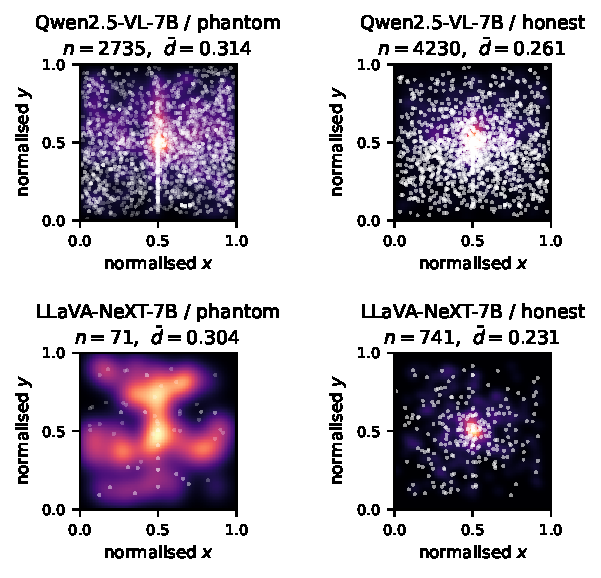
\includegraphics[width=\columnwidth]{figures/fig3_atlas.pdf}
\caption{Phantom vs.\ honest box-centre density, per model. Phantom
boxes sit noticeably further from the image centre.}
\label{fig:atlas}
\end{figure}

\paragraph{Detector (Fig.~\ref{fig:roc}, Table~\ref{tab:detector}).}
The full-feature LR reaches $\mathrm{AUROC}=0.916$ on Qwen
($n{=}6{,}965$) and $0.873$ on LLaVA ($n{=}812$), both exceeding
HALP's $0.787$. On Qwen the bbox geometry adds to the yes-token
confidence ($0.899\!\to\!0.916$); on LLaVA, geometry and confidence
overlap and are near-indistinguishable.

\begin{table}[!htbp]
\centering\small
\setlength{\tabcolsep}{4pt}
\begin{tabular}{llccc}
\toprule
\textbf{Model} & \textbf{Set} & $n$ & $\bar{d}_\text{center}$ & $\bar{A}$ \\
\midrule
Qwen2.5-VL-7B  & phantom & 2735 & 0.314 & 0.106 \\
Qwen2.5-VL-7B  & honest  & 4230 & 0.261 & 0.167 \\
LLaVA-NeXT-7B  & phantom &   71 & 0.304 & 0.189 \\
LLaVA-NeXT-7B  & honest  &  741 & 0.231 & 0.239 \\
\bottomrule
\end{tabular}
\caption{Atlas summary. Phantoms are further from centre and smaller
than honest boxes for both models.}
\label{tab:atlas}
\end{table}

\begin{figure}[!htbp]
\centering
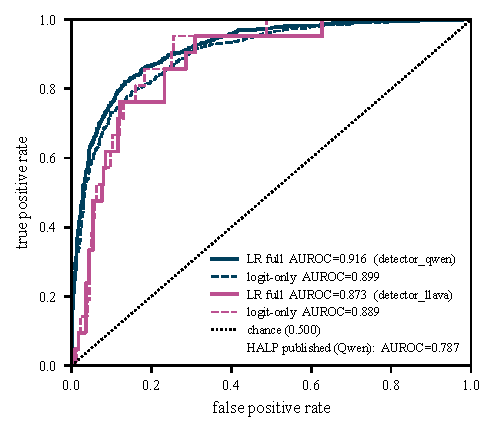
\includegraphics[width=\columnwidth]{figures/fig4_roc.pdf}
\caption{Detector ROC. LR on phantom-box features (solid) vs.\ a
logit-only baseline (dashed) vs.\ chance.}
\label{fig:roc}
\end{figure}

\begin{table}[!htbp]
\centering\small
\begin{tabular}{lcc}
\toprule
\textbf{Detector} & \textbf{Qwen2.5-VL-7B} & \textbf{LLaVA-NeXT-7B} \\
\midrule
Random                       & 0.500 & 0.500 \\
HALP (published)\cite{halp}  & 0.787 & --    \\
Logit only                   & 0.899 & 0.889 \\
LR full (ours)               & \textbf{0.916} & \textbf{0.873} \\
\bottomrule
\end{tabular}
\caption{Detection AUROC on stratified $70/30$ splits
($n{=}6{,}965$ Qwen; $n{=}812$ LLaVA). Our first-party detector
beats HALP's internal-feature detector on Qwen by $+12.8$ points.}
\label{tab:detector}
\end{table}

\paragraph{Analysis.} Qwen grounds on virtually every positive
($100\%$) while LLaVA grounds on only $19\%$, so LLaVA's yes-token
logprob already captures most of the separating signal and geometry
adds little. Qualitatively, phantoms cluster into three patterns
(Fig.~\ref{fig:failures}): \emph{oversized hedge boxes} that
half-cover the scene (typical for categories that rarely appear at
small scale in COCO, e.g.\ ``stop sign'', ``surfboard''),
\emph{peripheral boxes} pressed to a corner or edge of the image
(common for small-scale categories the model is less confident
about, e.g.\ ``scissors'', ``toilet''), and \emph{edge-clipped
boxes} whose boundary is flush with an image border (frequently
hallucinated on cluttered urban or kitchen scenes).
False negatives (phantoms missed by the detector) are dominated by
high-frequency COCO classes such as ``person'', ``chair'', and
``dining table'', for which the model emits plausibly sized and
centred boxes that blend in with honest examples. False positives
come from honest ``yes'' answers with small, off-centre objects
(truncations or crops) that coincidentally look phantom-like. This
indicates the atlas signal we exploit is informative but not a
single magic knob: the detector learns a multi-dimensional
decision boundary rather than a simple threshold on size or
position.

\paragraph{Limitations and future work.} Three caveats apply. First,
POPE draws its negatives from a fixed $80$-class COCO taxonomy, so
the atlas may not generalise to open-vocabulary hallucinations where
the imagined object lies outside this set. Second, we train and
evaluate on the same image distribution (COCO val2014); cross-domain
transfer to medical, satellite, or documentary imagery is untested.
Third, we model only two summary statistics of the phantom bbox --
centre distance and area -- whereas category-conditional priors or
aspect-ratio skew could plausibly tighten the detector further. A
natural follow-up is to extend the atlas to newer grounded VLMs
(Molmo, InternVL3) and richer benchmarks (HallusionBench, BEAF), and
to combine the first-party geometry signal with the internal-feature
signal of HALP~\cite{halp} to see whether the two are complementary
or redundant.

\begin{figure}[!htbp]
\centering
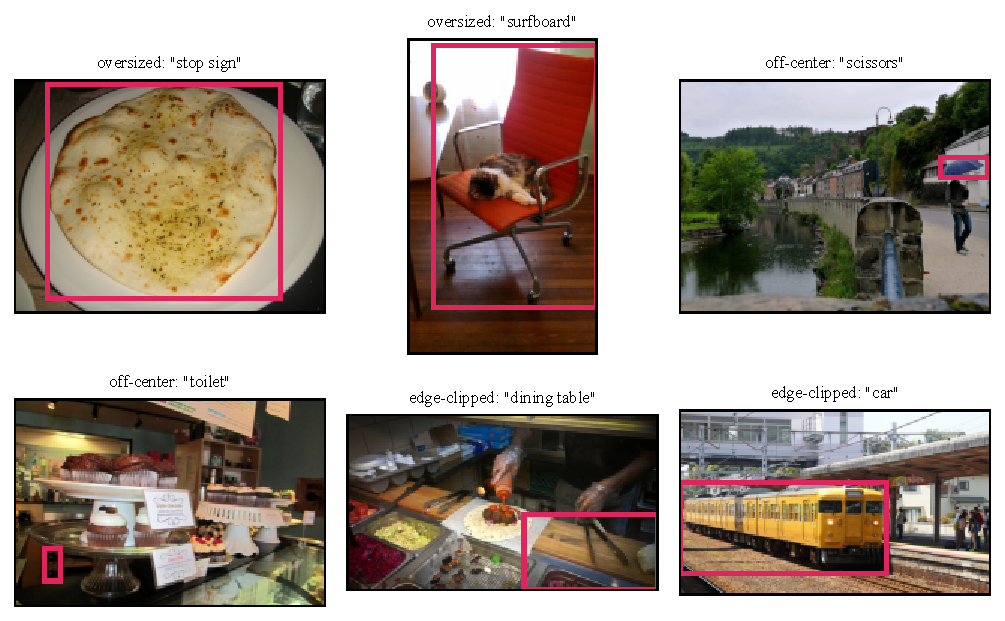
\includegraphics[width=\columnwidth]{figures/fig5_failures.pdf}
\caption{Three phantom failure modes: oversized (top), off-centre
(middle), edge-clipped (bottom).}
\label{fig:failures}
\end{figure}

%%%%%%%%% CONCLUSION
\section{Conclusion}

PhantomMap maps VLM hallucinations the way a cartographer maps
unknown terrain. Using only the VLM's public bbox interface on POPE,
we show that phantoms are placed with a predictable spatial signature
-- smaller, further from centre -- across two 7B-scale VLMs with very
different grounding recipes, and that this signature feeds a
training-free detector that exceeds the strongest
internal-feature baseline. \emph{Where} a hallucination is drawn
turns out to carry at least as much information as what it names, and
it is accessible to anyone with API access to the model. Because the
same features could help adversaries hide hallucinations, we release
code under an academic-use licence and add no new images to the
public domain; POPE inherits COCO's biases and so does our atlas.

\noindent
{\bf Acknowledgments.} We used Claude Opus 4.7 (Anthropic) for early
brainstorming and literature-scan sanity checks. We thank the authors
of POPE \cite{pope}, Qwen2.5-VL \cite{qwen25vl}, LLaVA-NeXT
\cite{llavanext}, and EAZY \cite{eazy} for making their code and data
publicly available. Shouyu Wang wrote the evaluation code and ran all
VLM experiments; Limeng Wang built the atlas visualisations, produced
the figures, and wrote the related work.

{\small
\bibliographystyle{ieee}
\bibliography{egbib}
}

\end{document}
